\chapter{Weitere entwickelte Ansätze}\label{weitere_ansaetze}
Um einen Vergleich des entwickelten Ansatzes zu weiteren Technologien aufstellen zu können, wurden zwei weitere Verfahren für die Implementierung der Entscheidungsfindung intelligenter Agenten verwendet. 
Die grundsätzliche Struktur der Dorfsimulation bleibt dabei erhalten. Die Entscheidungsfindung der Agenten dagegen ändert sich maßgeblich.
Es wurde ein regelbasierter sowie ein \ac{goap}-basierter Ansatz entwickelt. Im Folgenden werden diese vorgestellt.


\section{Regelbasierter Ansatz}
Für den regelbasierten Ansatz wurde die Klasse \inlinecode{ManualDecisionMaker} erstellt. Der Aufbau der Klasse ist in Abbildung \ref{fig:architecture_diagram_manualdecisionmaker} zu erkennen:

\begin{figure}[H]
\centering
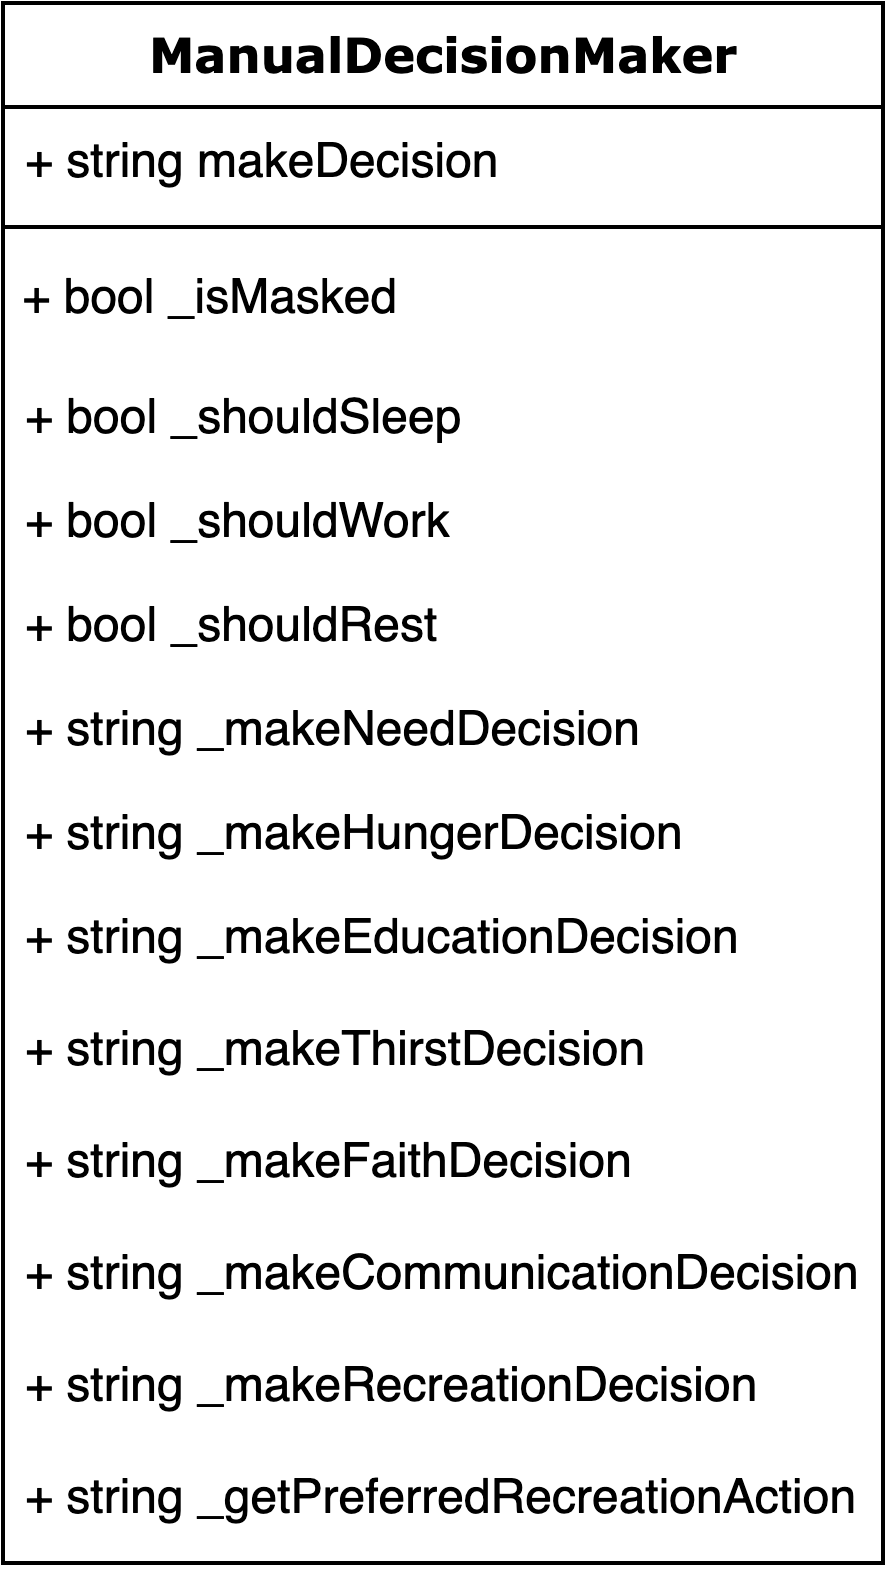
\includegraphics[scale=0.20]{images/village/architecture_diagram_manualdecisionmaker.png}
\caption{Methoden der Klasse \inlinecode{Manual Decision Maker}}
\label{fig:architecture_diagram_manualdecisionmaker}
\end{figure}

Der \inlinecode{ManualDecisionMaker} übernimmt die Entscheidungsfindung, indem er den Zustand des Agenten betrachtet und auf der Grundlage von bestimmten Regeln die beste Aktion auswählt. Die Klasse ersetzt im Architekturdiagram (siehe Abbildung \ref{fig:architecture_general}) die Rolle des externen Tensorflow-Backends welches für die Entscheidungsfindung zuständig ist. Die Klasse \inlinecode{NpcAgent} wird also weiterhin verwendet, alle Funktionen des ML-Agents-Frameworks werden aber deaktiviert. Da der \inlinecode{NpcAgent} bereits über alle nötigen Abhängigkeiten, Handler und Komponenten verfügt, wird der generelle Aufbau der Architektur nicht weiter verändert. Die Methode \inlinecode{requestModelOrManualDecision} ruft dann statt der ML-Agents-Funktion \inlinecode{RequestDecision} die Funktion \inlinecode{makeDecision} in der Klasse \inlinecode{ManualDecisionMaker} auf, um abhängig vom Zustand des Agenten Entscheidungen zu treffen. Die Funktion \inlinecode{makeDecision} ist im folgenden Listing \ref{lst:manual_decision_maker_make_decision} zu sehen:

\begin{minipage}{\linewidth}
\begin{lstlisting}[linewidth=16.4cm, label=lst:manual_decision_maker_make_decision, caption=Funktion \inlinecode{makeDecision} im \inlinecode{ManualDecisionMaker}, xleftmargin=1cm, basicstyle=\footnotesize]
public string makeDecision() {
    _mask = _npc.ActionMaskingHandler.getStringActionMask(_npc);

    if (_shouldSleep()) return NpcActions.SLEEP;
    if (_shouldWork()) return _npc.NpcState.AgentInfo.JobId;
    if (_shouldRest()) return NpcActions.RESTING;

    string action = _makeRecreationDecision();
    if (action != null) return action;

    action = _makeNeedDecision();
    if (action != null) return action;

    Debug.LogWarning("Could not find a good action for the agent. Choosing a random action that is not masked instead.");
    List<string> unmaskedActions = new List<string>();
    foreach (string actionId in NpcActions.ALL_ACTIONS) {
        if (!_mask.Contains(actionId)) unmaskedActions.Add(actionId);
    }
    if (unmaskedActions.Count != 0) {
        return unmaskedActions[Mathf.RoundToInt(Random.value * (unmaskedActions.Count - 1))];
    }
    Debug.LogWarning("Could not manage to find ANY actions for the agent! Choosing an action that IS MASKED instead.");
    return NpcActions.ALL_ACTIONS[Mathf.RoundToInt(Random.value * (NpcActions.ALL_ACTIONS.Length - 1))];
}
\end{lstlisting}
\end{minipage}

Eine Reihe von Bedingungen werden der Reihe nach mit absteigender Priorität abgearbeitet. Unter anderem wird dabei die Ausführbarkeit der Aktion geprüft, indem ermittelt wird, ob diese durch \inlinecode{\_mask} maskiert ist. Sobald eine Bedingung zutrifft, gibt die jeweils aufgerufene Funktion den Identifier einer Aktion in Form eines Strings zurück. Wenn der Rückgabewert \Fachbegriff{null} ist, wird die nächste Bedingung bearbeitet. Zunächst wird geprüft, ob der Agent schlafen, arbeiten oder ruhen muss.
Wenn keine dieser Bedingungen zutrifft, wird mittels \inlinecode{\_makeRecreationDecision} ermittelt, ob ein niedriger Wert für die Recreation des Agenten vorliegt, sodass dieser eine Freizeitaktivität ausführen sollte. Es werden ebenfalls die Attribute des Agenten mit einbezogen. Eine Liste aus allen Attributen des Agenten wird absteigend sortiert. Mit der Funktion \inlinecode{getPreferredAttributeAction} aus der Klasse \inlinecode{AttributeHandler} wird nun für jedes Attribut in der Liste nacheinander geprüft, ob die durch die Attribute des Agenten präferierte Aktion ausführbar ist.

Falls keine Recreation-Aktion gefunden wurde, werden schließlich die Bedürfnisse des Agenten betrachtet. Die entsprechende Funktion ist in Listing \ref{lst:manual_decision_maker_need_decision} zu finden. Ähnlich wie bei den Attributen wird eine Liste von allen Bedürfnissen sortiert, hier jedoch aufsteigend. Der Reihe nach wird dann in einem \Fachbegriff{switch-case} geprüft, ob die mit dem Bedürfniss verbundenen Aktionen ausführbar sind.

\begin{minipage}{\linewidth}
\begin{lstlisting}[linewidth=16.4cm, label=lst:manual_decision_maker_need_decision, caption=Funktion \inlinecode{makeNeedDecision} im \inlinecode{ManualDecisionMaker}, xleftmargin=1cm, basicstyle=\footnotesize]
private string _makeNeedDecision() {
    List<KeyValuePair<string, float>> needs = new List<KeyValuePair<string, float>>();
    foreach (string needType in NpcState.ALL_NEEDS) {
        needs.Add(new KeyValuePair<string, float>(needType, _npcState.getNeedByType(needType)));
    }
    needs.Sort((x, y) => x.Value.CompareTo(y.Value));

    foreach (KeyValuePair<string, float> need in needs) {
        string decision = null;
        switch (need.Key) {
            case NpcState.NEED_HUNGER:
                decision = _makeHungerDecision();
                break;
            case NpcState.NEED_THIRST:
                decision = _makeThirstDecision();
                break;
            case NpcState.NEED_EDUCATION:
                decision = _makeEducationDecision();
                break;
            case NpcState.NEED_COMMUNICATION:
                decision = _makeCommunicationDecision();
                break;
            case NpcState.NEED_FAITH:
                decision = _makeFaithDecision();
                break;
        }
        if (decision == null) continue;
        else return decision;
    }
    return null;
}
\end{lstlisting}
\end{minipage}

Wenn auch bei diesem Vorgehen keine gültige Aktion gefunden wird, wird eine zufällige Aktion gewählt, die nicht maskiert ist. Wenn auch das scheitert, wird eine zufällige maskierte Aktion ausgewählt. Alternativ könnte der Agent ebenfalls so lange keine Aktion ausführen, bis eine Aktion verfügbar ist.







\section{Goal Oriented Action Planning}
Weiterhin wurde ein Ansatz entwickelt, der auf \ac{goap} basiert (siehe Kapitel \ref{goap}). Nicht alle Features des Dorfes, die im Kapitel \ref{entwicklung_dorf} vorgestellt wurden, sind in diesem Verfahren funktionsfähig. Es handelt sich eher um ein Proof-Of-Concept, das das generelle Vorgehen der Implementierung von \ac{goap} dokumentieren soll.

Im Folgenden wird die Architektur des Ansatzes beschrieben. Zunächst wird auf die wichtigsten Komponenten der verwendeten Bibliothek eingegangen.


\subsection{Verwendete GOAP-Bibliothek}
Für die Implementierung wurde die Open Source-Bibliothek \Fachbegriff{GOAP} genutzt \cite{goap_library}. Zunächst werden die wichtigsten Klassen der Bibliothek beschrieben.

\subsubsection{GoapAction}
Die Klasse \inlinecode{GoapAction} beschreibt eine ausführbare GOAP-Aktion, die bestimmte Bedingungen erfordert und Effekte verursacht. Sie dient als Grundlage für die Erzeugung des Aktionsbaumes, der den Weg von einem Startpunkt über Aktionen zu einem Ziel bzw. Goal beschreibt.

Im Konstruktor der Klasse werden Effekte hinzugefügt. Diese werden in der Klasse \inlinecode{Effects} definiert und im Feld \inlinecode{List<string> effects} gespeichert. Äquivalent dazu werden in der Variablen \inlinecode{preconditions} Bedingungen festgehalten. Weiterhin muss eine Reichweite \inlinecode{requiredRange} festgelegt werden. Später wird dieser Wert für die Navigation des Agenten zum Zielort benutzt. In dem Feld \inlinecode{cost} werden darüber hinaus die Kosten für die Aktion festgelegt.
Schließlich muss die Funktion \inlinecode{Perform} überschrieben werden, um die eigentlich Aktion auszuführen - beispielsweise das Warten eines Agenten für einen bestimmten Zeitraum an einem bestimmten Ort.

\subsubsection{GoapGoal}
Um das Ziel eines Agenten zu beschreiben, wird in der Klasse \inlinecode{Goal} ein Identifier für ein neues Goal anhand einer String-Konstante erzeugt. Dieses Ziel wird einer bestimmten Aktion zugewiesen, deren Ausführung das Erreichen des Ziels beschreiben soll. Die Zuweisung erfolgt in dem Feld \inlinecode{goal} der \inlinecode{GoapAction}.
Weiterhin muss eine neue Klasse erstellt werden, die von der Klasse \inlinecode{GoapGoal} erbt und direkt mit dem definierten Ziel verbunden ist. Die entsprechende String-Konstante, die das Ziel beschreibt, ist ein Parameter für den Konstruktor des \inlinecode{GoapGoal}. Nun wird eine Liste aller Aktionen erstellt, die das entsprechende Ziel haben.

\subsubsection{GoapAgent}
Die Klasse \inlinecode{GoapAgent} verwaltet alle Aktionen und Goals des Agenten. Der Aktionsbaum für die Entscheidungsfindung des Agenten wird hier aufgebaut.
Zunächst werden alle verfügbaren Aktionen mithilfe der Funktion \inlinecode{AddAction} hinzugefügt. Ebenfalls werden alle erzeugten Goals in das Feld \inlinecode{Dictionary<string, GoapGoal>} mit aufgenommen.
Für jedes der Goals wird nun anhand der Effekte und Bedingungen der Aktionen ein Aktionsbaum erzeugt. Mithilfe der jeweils definierten Kosten kann dann der kürzeste Weg zum Ziel berechnet werden, der mit den niedrigsten Kosten verbunden ist.
Zusätzlich muss die Funktion \inlinecode{Move} überschrieben werden, um eine Navigation des Agenten zum Zielort der Aktionen zu ermöglichen.


\subsection{Architektur}
% wie wird das überhaupt in die bestehende simulation integriert?
In der \inlinecode{GameAcademy} kann durch den Parameter \inlinecode{useGoap} bestimmt werden, ob \ac{goap}-basierte Agenten anstelle eines trainierten Modells für \ac{reinforcement_learning}-basierte Agenten verwendet werden sollen. Die GOAP-Implementierung nimmt hier, ähnlich wie bereits der \inlinecode{ManualDecisionMaker} im vorherigen Abschnitt, die Rolle des externen Tensorflow-Backends ein, um Entscheidungen für den Agenten in Abhängigkeit von seinem Zustand zu treffen. Obwohl \ac{goap}-basierte Agenten verwendet werden, müssen Agenten vom Typ \inlinecode{NpcAgent} erzeugt werden, da die Komponenten dieser Klasse für die \ac{goap}-Agenten verwendet werden. Lediglich die eigentliche Entscheidungsfindung der \inlinecode{NpcAgent}s wird deaktiviert. Dafür wird in der Funktion \inlinecode{requestModelOrManualDecision} der Klasse \inlinecode{NpcAgent} der entsprechende Parameter geprüft.
In der Funktion \inlinecode{\_initAgent} in der Klasse \inlinecode{Village} wird ein einzelner \inlinecode{NpcAgent} initialisiert. Zusätzlich werden dort \ac{goap}-Agenten vom Typ \inlinecode{NpcGoapAgent} erzeugt, wie im Listing \ref{lst:create_goap_agents} zu sehen:

\begin{minipage}{\linewidth}
\begin{lstlisting}[linewidth=16.4cm, label=lst:create_goap_agents, caption=Erzeugung \ac{goap}-basierter Agenten \inlinecode{NpcGoapAgent}, xleftmargin=1cm]
if (GameAcademy.USE_GOAP) {
    yield return Ninja.JumpToUnity;
    goapAgent = npcAgent.gameObject.AddComponent<NpcGoapAgent>();
    VillageGoapActionAdder goapActionAdder = new VillageGoapActionAdder();
    yield return goapActionAdder.createGoapActions(npcAgent, goapAgent, _villageInfo);
    goapAgent.Init(npcAgent, goapActionAdder.GoapActions);
}
\end{lstlisting}
\end{minipage}

Die Funktion \inlinecode{Init} der Klasse \inlinecode{NpcGoapAgent} initialisiert den Agenten mit zwei benötigten Parametern, dem verbundenen \inlinecode{NpcAgent} und einer Liste der möglichen Aktionen \inlinecode{List<GoapAction>}. Weiterhin werden dort alle Goals des Agenten hinzugefügt.
Die Methode \inlinecode{Move} wird wie folgt überschrieben und zusätzlich eine Funktion \inlinecode{\_moveFinished} hinzugefügt:

\begin{minipage}{\linewidth}
\begin{lstlisting}[linewidth=16.4cm, label=lst:move_goap_agent, caption=Implementierung der Funktion \inlinecode{Move} in der Klasse \inlinecode{NpcGoapAgent}, xleftmargin=1cm]
protected override void Move(GoapAction nextAction) {
    Vector3 moveAgentPosition = _npcAgent.MoveHandler.NavAgent.transform.position;
    Vector3 moveAgentDestination = _npcAgent.MoveHandler.NavAgent.destination;
    Vector3 nextActionDestination = nextAction.target.transform.position;
    if (Equals(moveAgentDestination, nextActionDestination) ||
        Equals(moveAgentPosition, nextActionDestination)) return;

    _npcAgent.VillageInfo.changeAmountMoving(true);
    _npcAgent.MoveHandler.moveAgent(nextAction.target.transform.position, nextAction.GetType().ToString(), null);
}

private void _moveFinished() {
    _npcAgent.VillageInfo.changeAmountMoving(false);
}
\end{lstlisting}
\end{minipage}
Für die Bewegung des Agenten wird also der \inlinecode{MoveHandler} des \inlinecode{NpcAgent} verwendet. Falls das Ziel des Agenten bereits mit dem Ziel der nächsten Aktion übereinstimmt, befindet sich der Agent bereits auf dem Weg zum Ziel, sodass ein erneuter Aufruf von \inlinecode{moveHandler.move} nicht nötig ist. Das gilt auch für den Fall, dass der Agent sich bereits an der Zielposition befindet. Sobald der Bewegungsvorgang abgeschlossen wurde, wird die Funktion \inlinecode{\_moveFinished} aufgerufen, um im UI die korrekte Anzahl bewegender Agenten zu zeigen.
Zusätzlich wird die Getter-Funktion \inlinecode{ActiveActionInRange} überschrieben:

\begin{minipage}{\linewidth}
\begin{lstlisting}[linewidth=16.4cm, label=lst:activeactioninrange_goapagent, caption=Implementierung der Getter-Funktion \inlinecode{ActiveActionInRange} in der Klasse \inlinecode{NpcGoapAgent}, xleftmargin=1cm]
protected override bool ActiveActionInRange {
    get {
        if (ActiveAction == null) return true;
        float distance = Vector3.Distance(transform.position, ActiveAction.target.transform.position);
        return distance <= GameAcademy.AGENT_STOPPING_DISTANCE;
    }
}
\end{lstlisting}
\end{minipage}

\inlinecode{ActiveActionInRange} wird regelmäßig aufgerufen um zu prüfen, ob ein Agent an der Zielposition der aktuellen Aktion angekommen ist. Wenn der Abstand des Ziels zum Agent kleiner ist als die \Fachbegriff{Stopping Distance} des Agenten \inlinecode{GameAcademy.AGENT\_STOPPING\_DISTANCE}, so ist die Bewegung abgeschlossen und die Aktion kann ausgeführt werden.

Nun muss eine Reihe von Goals und Aktionen definiert werden, um für die jeweiligen Goals Aktionsbäume aufzubauen. Zunächst wurde für jedes Bedürfnis des Agenten ein Goal definiert. Dafür wurden die Klassen \inlinecode{CommunicationGoapGoal}, \inlinecode{EducationGoapGoal}, \inlinecode{ExhaustionGoapGoal}, \inlinecode{FaithGoapGoal}, \inlinecode{HungerGoapGoal}, \inlinecode{RecreationGoapGoal}, \inlinecode{SleepGoapGoal}, \inlinecode{ThirstGoapGoal} und \inlinecode{WorkGoapGoal} erzeugt, sowie entsprechende Konstanten für die jeweiligen Identifier der Goals.
Anschließend wurde für die grundsätzlichen Aktionen des Agenten, die zuvor durch ActionPlans beschrieben wurden, eigene \inlinecode{GoapAction}s entwickelt. Da in ActionPlans mehrere Subaktionen genutzt werden können, was in dem Fall von \inlinecode{GoapAction}s nicht möglich ist, wurden zusätzlich weitere Aktionen erstellt, um die einzelnen in den ActionPlans definierten Teilaktionen zu modellieren. Die definierten Aktionen können im Unterordner \inlinecode{GoapActions} betrachtet werden.



